\documentclass[a4paper]{article}

\usepackage[english]{babel}
\usepackage[utf8x]{inputenc}
\usepackage{amsmath}
\usepackage{amsfonts}
\usepackage{graphicx}
\usepackage[]{algorithm2e}
\usepackage[colorinlistoftodos]{todonotes}

\title{CS 5785 -- Applied Machine Learning -- Lec.\ 13}
\author{Prof.\ Nathan Kallus \\Scribe: TBD}
\date{Oct.\ 17, 2017 (Under construction)}

\begin{document}
\maketitle

\section{Principal Components Analysis (PCA)}

\begin{figure}
\centering
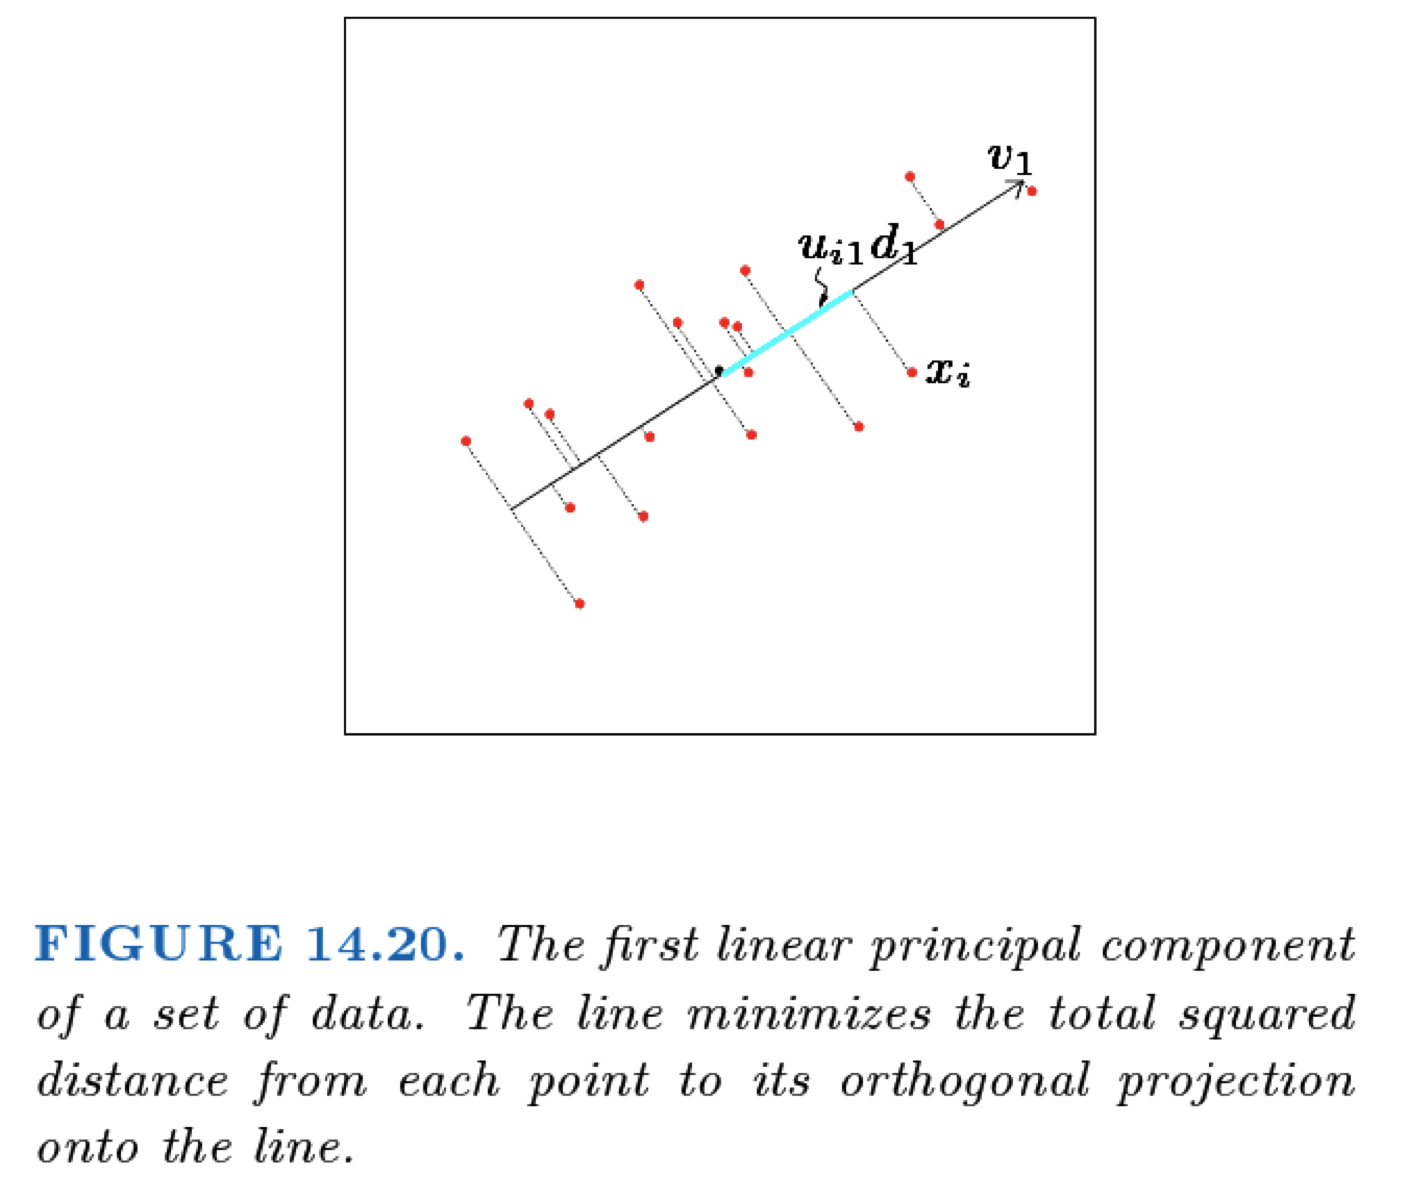
\includegraphics[width=1.0\textwidth]{TwoDimReduction.png}
\caption{\label{fig:2DimReduction} Dimensionality reduction from 2 dimensions to 1 dimension}
\end{figure}


\begin{figure}
\centering
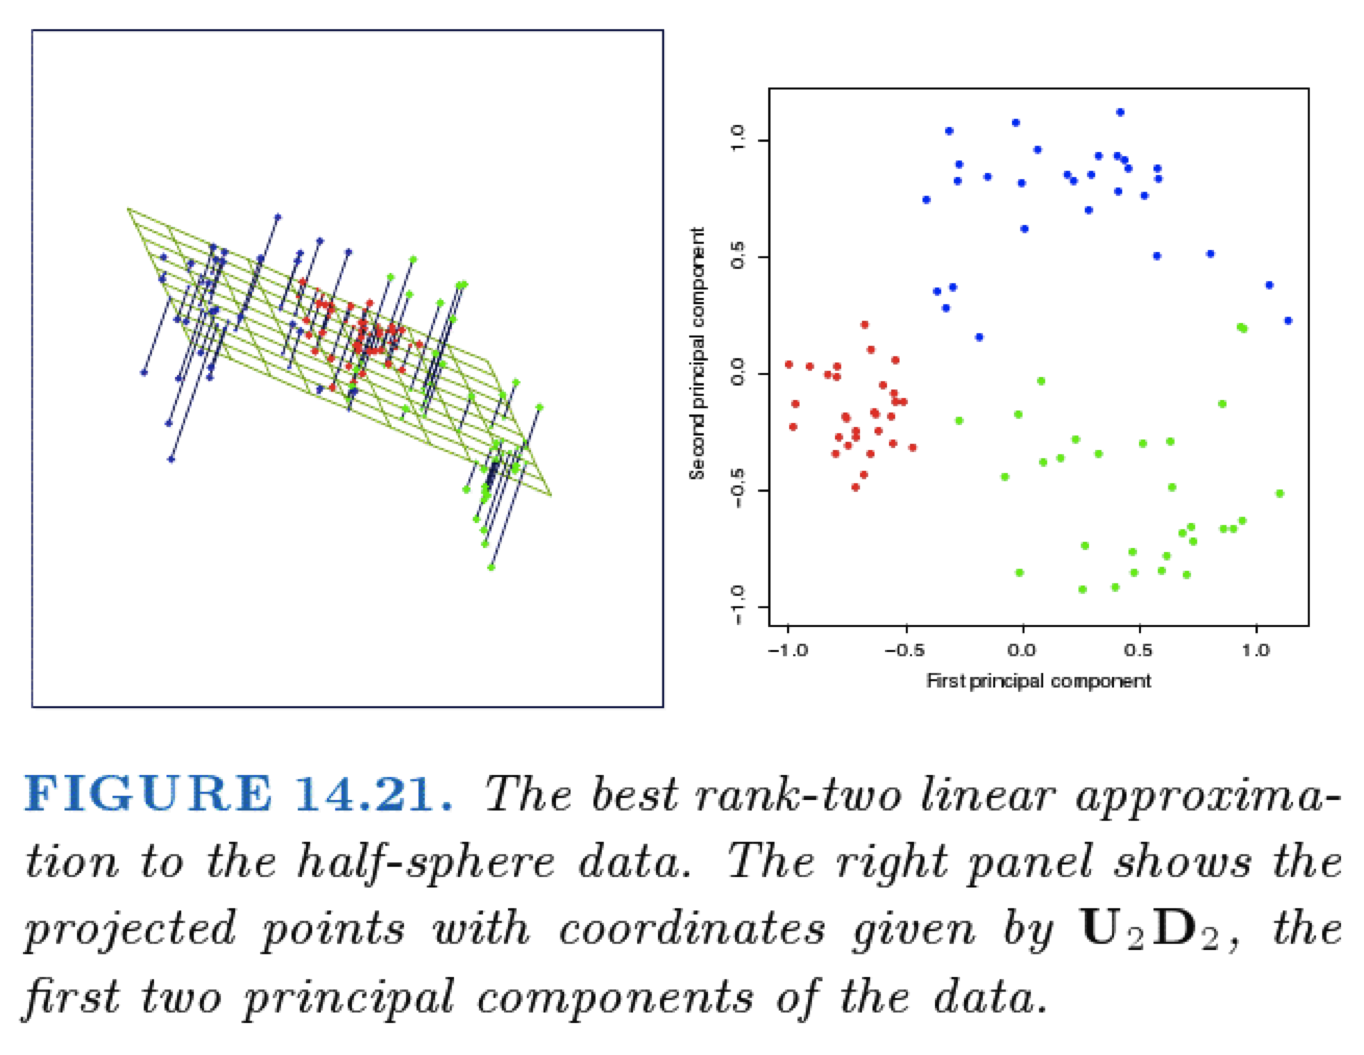
\includegraphics[width=1.0\textwidth]{ThreeDimReduction.png}
\caption{\label{fig:3DimReduction}Dimensionality reduction from 3 dimensions to 2 dimension}
\end{figure}

\subsection{Recap}
PCA is an unsupervised dimensionality reduction technique. To use it, we start by stacking the feature vectors ${x_i}$ into a matrix $\mathbf{X}\in \mathbb{R}^{N\times p}$. PCA is used to discover axes of variation in a dataset. In the following discussion, we assume that the data is centered, i.e., $\bar{x}=0$, which we can do by setting $x_i = x_i -\bar{x}$ for all $i$. PCA requires us to find the eigenvectors of the sample covariance matrix of the feature vectors, which is given by: $$\mathbf{S} = \frac{1}{N}\mathbf{X}^\top\mathbf{X}\in\mathbb{R}^{p\times p}$$
We sometimes also refer to the quantity $\mathbf{X}^\top\mathbf{X}$, i.e., without the $1/N$ or $1/(N-1)$ scale factor, as the covariance matrix, but technically it is the ``scatter matrix.''
We compute the SVD, $X=\mathbf{U}\mathbf{D}\mathbf{V}^\top$. The columns of $\mathbf{UD}$ are the principal components of $\mathbf{X}$. The singular values $d_1 \geq \ldots \geq d_p \geq 0$ capture the variance along each principal axis.

Figure \ref{fig:2DimReduction} is an example of a dimensionality reduction where $p=2$ and $q=1$. In Figure \ref{fig:3DimReduction}, $p=3$ and $q=2$. 
For simplicity, assume we have a \textit{centered} set of data, i.e., $\bar{x}=0$.

As an aside of ``punk stats,'' it may be helpful to think of 2 different types of datasets: clumpy and manifold-y. Clumpy datasets would use methods like k-means, GMM with EM algorithm, etc and are well represented by tokens/cluster centers.  Manifold-y datasets, where instead of clusters there are curves and low dimensional coordinate systems, methods like PCA would be used with these datasets if the manifold is known. 

\subsection{MNIST Digits}

\begin{figure}
\centering
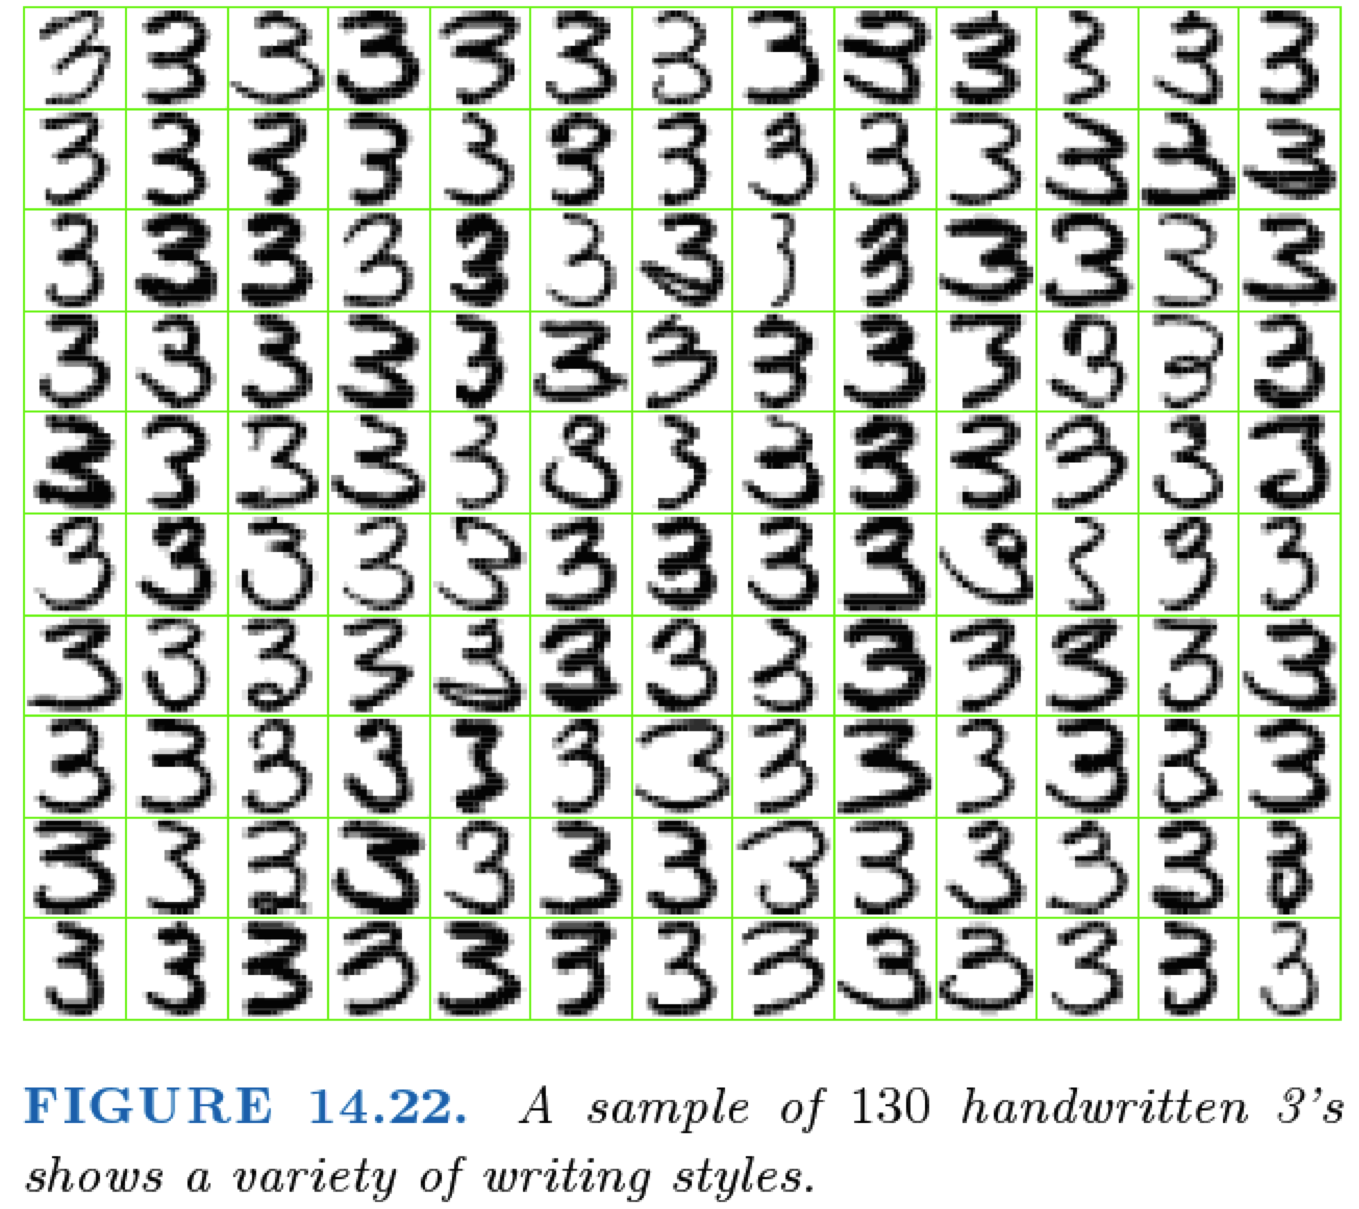
\includegraphics[width=1.0\textwidth]{Figure1422.png}
\caption{\label{fig:1422}}
\end{figure}

We can think of images of handwritten digits as living on a manifold since it's plausible that we could express one instance as a linear (weighted) combination of other instances. If we look at Figure \ref{fig:1422} we can see a collection of instances of the digit 3 drawn by different people. Like $K$-means, PCA operates on a set of vectors, which means we need to transform the digit images, each of which are $28\times 28$ pixel images, into to vectors. The way we do that is by concatenating the rows or columns to create a single vector of length $784$.  When we run either $K$-means or PCA on these vectors we obtain vectors as a result which we can then reschape or ``un-concatenate'' for purposes of visualization.

\begin{figure}
\centering
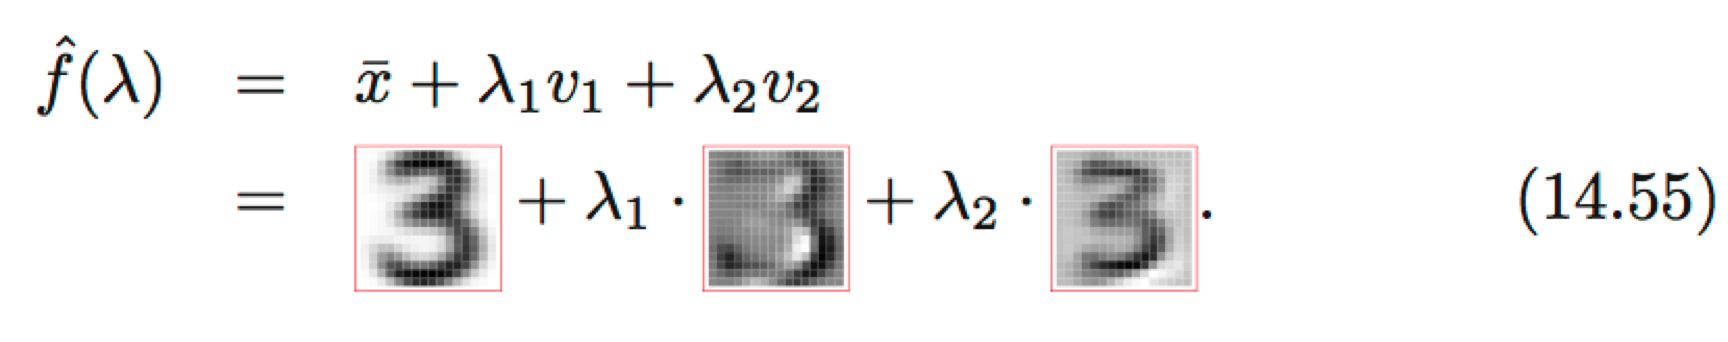
\includegraphics[width=1.0\textwidth]{Figure1455.png}
\caption{\label{fig:1455}}
\end{figure}

Given a set of digits (such as those in Figure \ref{fig:1422}), each digit can be represented by a linear combination of the mean of all the digit examples plus a constant times the first principal component and the same for the second principal component and so on.  Figure \ref{fig:1455} shows an example of a digit being represented by the mean, $\bar{x}$, and a linear combination of the two leading principal components, $v_1$ and $v_2$. Each principal component represents slight changes relative to the mean (like stretching, rotation or stroke dilation). 

\begin{figure}
\centering
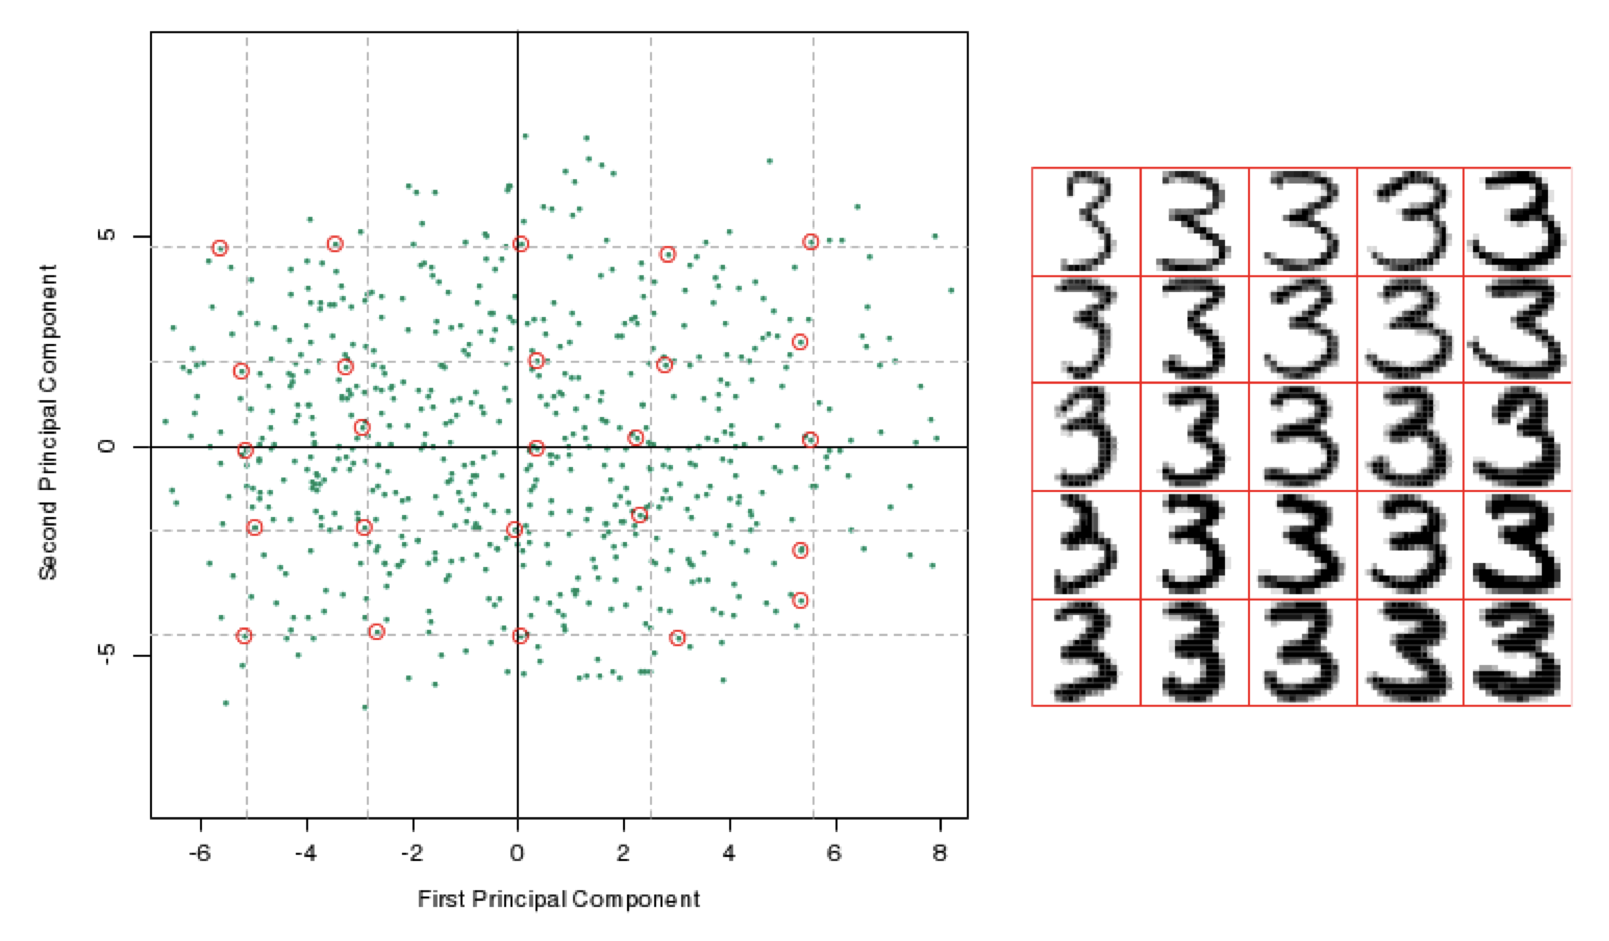
\includegraphics[width=1.0\textwidth]{Figure1423.png}
\caption{\label{fig:1423} Dimensionality reduction from 784 dimensions to 2 dimensions using PCA.}
\end{figure}

Figure \ref{fig:1423} shows the result of performing PCA on a set of thousands of digit $3$'s and keeping only the $2$ strongest principal components. The figure also shows how picking $15$ examples scattered on this 2 dimensional space can inform us of the type of linear change that each principal component captures. Each red dot on the graph corresponds to the relative digit depicted on the right. The digits are reconstructed from the principal components as specified in Figure \ref{fig:1455}. A closer look at the digits reveals that the principal component represented by the $y$ axis captures the stroke strength and the one represented by the $x$ axis captures the curvature of the digit.

\subsubsection{Eigenfaces}

\begin{figure}
\centering
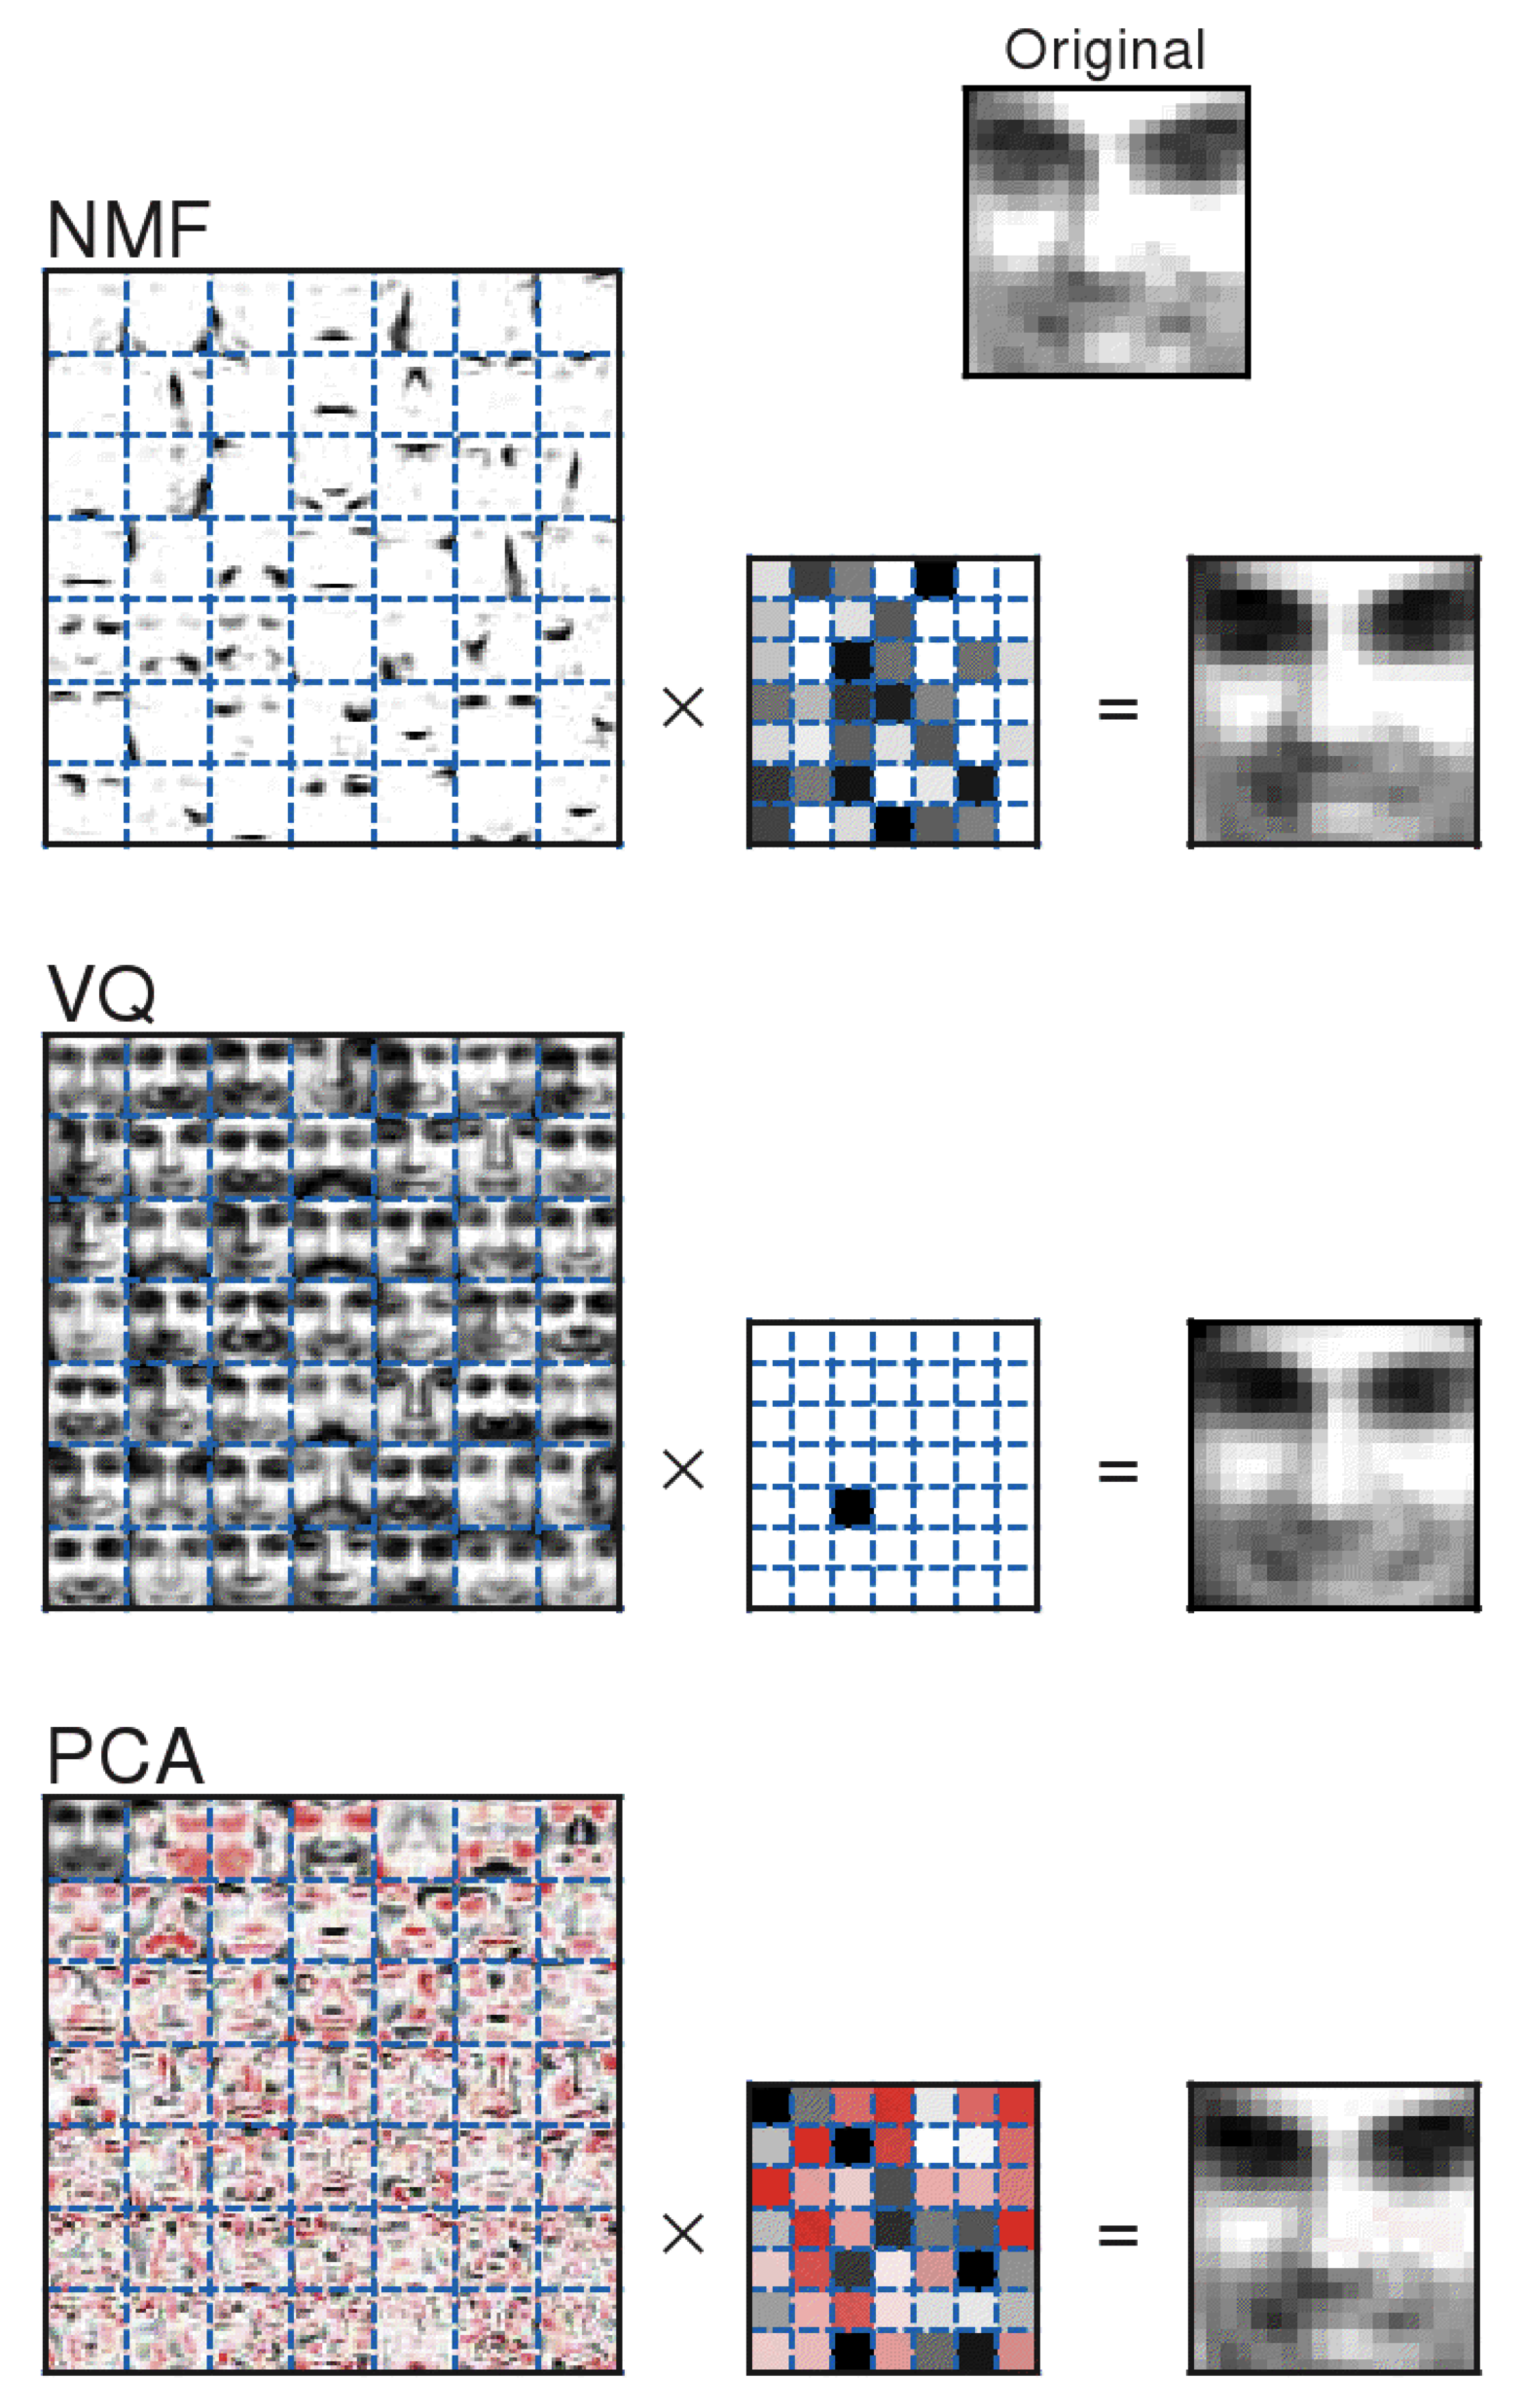
\includegraphics[width=1.0\textwidth]{Figure1433.png}
\caption{\label{fig:1433} Representing faces using dimensionality reduction techniques. Each sample face is a $19\times 19$ array, and the algorithms used $N=2,429$ training examples.  In the PCA example, negative values are shown in red/pink.}
\end{figure}

At the bottom of Figure \ref{fig:1433} we can see an example of PCA used for depicting faces. The top left part of the matrix on the left represents the mean face. Each of the other sections of this matrix represents a prinicipal component (where the black ranges represent positive values and the red ranges represent negative values). The $2$-D array we use to multiply the matrix by shows the constants we multiply each principal component by to get the  $48$ dimension approximation to the origianl face - The PCA reconstruction of this face. If we look closely we notice that the top left constant in this $2$-D array is black, meaning $1$, which will always be true because as we saw in Figure \ref{fig:1455} the mean appears once in every reconstructed sample.

\subsubsection{Uses of PCA}
There are a few possible uses for PCA that take advantage of the approximated representation of each sample as a $q$ sized vector:
\begin{itemize}

\item \textbf{Compression} We use less space to store the samples, since each reconstructed sample is shorter than the original. In Figure \ref{fig:1423} we have examples of digits that originally were represented by vectors of length $784$ and now are represented by vectors of length $2$.

\item \textbf{Recognition} After running PCA and keeping only the most meaningful components we have a shorter representation for each face. Two face images that have relatively close principal components might belong to the same person. In other words the \textit{dot product} of the $2$ samples with the principal components would result in similar vectors for samples belonging to the same person.

\item \textbf{Denoising} The smaller principal components that were removed during the dimensionality reduction might contain noise instead of meaningful, useful and interesting information. By removing them we denoise the given sample set.

\end{itemize} 

\section{Non-Negative Matrix Factorization (NMF)}
One aspect of PCA that may be undesireable in some cases is that it leaves the basis functions and coefficients free to swing into negative values, as seen by the amount of pink in Figure \ref{fig:1433}. This means that when we reconstruct samples using PCA some of the principal components cancel out part of other principal components, in a manner analogous to Fourier Series. A lot of the measurements of practical interest to us are non-negative. Nonnegative Matrix Factorization (NMF) takes this into consideration and uses this assumption to create a different method of dimensionality reduction (Lee \& Seung, 1999).
Given an $N\times p$ matrix, where each row represents a sample in our sample set, we use the approximation $\mathbf{X}\approx \mathbf{WH}$, where:
\begin{itemize}
\item $\mathbf{W}\in\mathbf{R}^{N\times r}$
\item $\mathbf{H}\in\mathbf{R}^{r\times p}$
\item $r \leq \max(N,p)$
\item Assume $x_{ij},w_{ik},h_{kj} \geq 0$, i.e., everything is nonnegative.
\end{itemize}

Find $\mathbf{W}$ and $\mathbf{H}$ by maximizing the log likelihood for a model in which $x_{ij}$ has a Poisson distribution with mean $\left(\mathbf{WH}\right)_{ij}$:
$$L(\mathbf{W},\mathbf{H})=\sum_{i=1}^N \sum_{j=1}^p \left[ x_{ij}\log\left(\mathbf{WH}\right)_{ij}-\left(\mathbf{WH}\right)_{ij}\right]$$

We will skip the discussion about how they arrived at this objective function. They use the following alternating algorithm to find a local maximum of $L(\mathbf{W},\mathbf{H})$:
$$w_{ik} \quad\leftarrow\quad w_{ik} \frac{\sum\limits_{j=1}^p h_{kj}x_{ij}/\left(\mathbf{WH}\right)_{ij}}{\sum\limits_{j=1}^p h_{kj}}$$
$$h_{kj} \quad\leftarrow\quad h_{kj} \frac{\sum\limits_{i=1}^N w_{ik}x_{ij}/\left(\mathbf{WH}\right)_{ij}}{\sum\limits_{i=1}^N w_{ik}}$$

Let us look at Figure \ref{fig:1433} again. It is clearly noticeable that in NMF all the basis images (on the left) and coefficients (on the right) are non-negative, since there are no shades of red. Each basis image represents part of a face, a feature, like glasses, beards, higher cheek bones, etc.\\

\subsection{Topic Modeling}
One application of NMF is \textit{topic modeling} in a collection of documents. Intuitively, given that a document is about a particular topic, one would expect particular words to appear in the document more or less frequently. In NMF topic modeling each document is represented by a \textit{bag of words}, a vector where each index correxponds to a word and the value to the number of times the words appear in the document. Since the vectors, which are just word-count histograms, are counting word occurences, they are non-negative by definition. Each topic is represented by a vector, similar to the basis images in the example shown in Figure \ref{fig:1433}, and each document can be described as a superposition of these components, all with nonnegative weights.  In practice, Latent Dirichlet Allocation is a more commonly used technique for document topic modeling.

\subsection{Sparsity}
If we look again at Figure \ref{fig:1433} we can see that representing a sample from the sample set using VQ is clearly cheaper in space than using the other methods, since it uses 1 value only. We call this a \textit{sparse} representation. VQ is the sparsest method but also the least accurate. If we regard the example in Figure \ref{fig:1433} as a way for Cornell campus security to cheaply represent the pictures of each student that using VQ each new student would be represented by the picture of the closest matched basis image from last year, clearly not a good enough estimation. In the other two cases, a new student would be represented by the mean face from last year (which given a large enough sample set shouldn't change much) and a linear combination of the basis images/principal components which is relatively unique to him.

In our case, sparsity means the number of zeros in the linear combination representing each sample. As stated before VQ is clearly the sparsest between the three, but between NMF and PCA, NMF is sparser. This because as we explained earlier, PCA hinges on the fact that the different principal components rely in part on cancellation effects. As such the linear combination is full of positive and negative values that balance to the final result. NMF on the other hand adds non-negative features only in the cases where they are relevant and there is no mutual cancellations so the resulting vector is sparser. 

\subsubsection{Cleve Moler's example of Sparsity}
``I'm thinking of two numbers whose average is 3. What are the numbers?''  Clearly, there is not enough information to answer the question definitively, but most people will answer ``$2$ and $4$.'' There are, of course, an infinite number of possible answers, the fact that most people would still give the same answer implies that there is some kind of \textit{regularization} on the solution that people perform when answering the question, in particular, one that picks a pair of numbers equidistant and not too far from the average.

The problem has the form $\mathbf{A}y=b$ with $\mathbf{A}=[0.5,0.5]$ and $b=3$. Possible solutions are: $y=[2,4]$, $y=[1,5]$, $y=[3,3]$ and $y=[0,6]$. The solution $y=[0,6]$ is the sparsest one, since half of its values are zero.

\subsubsection{Compressive Sensing}
\textit{Compressive Sensing} approaches seek the solution with minimum $\ell_0$ norm, which counts the non zero elements in a vector. The $\ell_0$ norm leads to very difficult combinatorial optimization problems. Donoho, Cand\`{e}s and Tao have shown that one can use the $\ell_1$ norm, the sum of absolute values,  instead of the $\ell_0$ norm and get basically the same solution. This permits a solution via linear programming. What we gain by choosing sparser solutions is the ability to recreate samples accurately using less information.

\end{document}
